\scanpage{72}
\begin{flushright}\handwritten{22.7.961}\end{flushright}

\begin{center}Commentair\deleted{\unsure{a}}es sur l'article de A.Delzant sur les formes quadratiques.\end{center}

Du point de vue rédaction;

a) Il est très confusant de faire semblant de traiter en même temps la carc. $\handwritten{\ne}2$ et la car. 2. Pour l'instant, même les structures qui entrent en jeu sont d'espèce différente, et le traitement des deux cas est vraiment différent. Si donc tu n'arrives pas à une théorie commune satisfaisante, laisse tomber la car.2, ou met\inserted{\handwritten{s}} dans un numéro à part ce que\deleted{\unsure{x}} tu sais en dire.

b) Contrairement à ce que suggère la lecture de l'article, le rôle des $\handwritten{\lambda}$-structures dans la théorie est pratiquement nul, dû\deleted{t} au fait sans doute que la filtration naturelle de l'anneau des classes de formes quadratiques n'est autre que celle définie par les puissances de l'idéal d'augmentation. On récupère trivialement la $\handwritten{\lambda}$-structure sur la forme explicite dudit anneau, et il suffit de le faire à la fin.

\deleted{\unsure{c)|a)}} Du point de vue math., je suggère comme programme minimum raisonnable le suivant, qui est à portée immédiate:

1) \uline{Structure de l'anneau} $Q(A)$ \uline{des classes de formes quadratiques sur} $A$, ou pour l'instant $A$ va être un corps de caractéristique $\handwritten{\ne}2$. Pour $a\handwritten{\in}A^{\handwritten{*}}$, soit $\handwritten{\varphi}_a$ la classe de la forme quadratique $\handwritten{at^2}_{a}$, elle ne dépend que de $a\bmod A^{\handwritten{*2}}$, d'où un homomorphisme de
\[
D(A)=A^{\handwritten{*}}/A^{\handwritten{*2}}=H^{\handwritten{1}}(A,\underline{Z}/2\underline{Z})
\]
dans $Q^{\deleted{\unsure{2|1}}}(A)^{\handwritten{*}}$, notée aussi $a\handwritten{\to\varphi}_a$, d'où un homomorphisme
\[
\handwritten{\varphi:}\ \underline{Z}(D)\handwritten{\longrightarrow}Q(A)
\tag*{\handwritten{(*)}}
\]
où $\underline{Z}(D)$ est l'algèbre du groupe $D=D(A)$, à coéfficients dans $\underline{Z}$. On prouvera alors le théorème suivant:

\uline{L'homomorphisme précédent est surjectif}, \uline{son noyau est} \deleted{formé \unsure{du|des}} \uline{le sous-groupe engendré par les} $e_a+\unsure{e|a}_b-e_{a'}-e_{b'}$, \uline{pour} $a,b,a',b'\handwritten{\in}D$ \uline{tels que} $\handwritten{\varphi}_a+\handwritten{\varphi}_b=\handwritten{\varphi}_{a'}+\handwritten{\varphi}_{b'}$. D'après un théorème de Witt, cette dernière relation équivaut aussi à dire que les formes des deux membres ont mêmes invariants, ce qui s'écrit plus simplement
\reversemarginpar
\margin{\handwritten{?}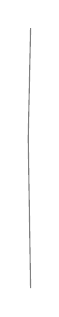
\begin{tikzpicture}[baseline=0pt]\draw[gray] (0.4,-1.7)--(0.37,0.2)--(0.4,1.6);\end{tikzpicture}}
\normalmarginpar
\[
a+b=a'+b'\ ,\quad a.b=a'.b'
\]
où $D$ est écrit additivement, et où le produit $a.b$ est le cup-produit, à valeurs dans
\[
B=H^{\handwritten{2}}(A,\underline{Z}/2\underline{Z})
\]
% archive sheet number: 71
